\section{PDF Vorstellung}
Das PDF Dateiformat steht für Plattformunabhängigkeit, Hardwareunabhängigkeit, Konsistenz in Formatierung und Layout und soll ein möglichst originalgetreues Druckergebnis liefern. Der Leser soll ein PDF Dokument immer nach dem Prinzip \gls{wysiwyg} (What You See Is What You Get) in der Form betrachten und ausdrucken können wie es vom Ersteller des Dokuments festgelegt wurde.
\par
PDF wurde im Jahr 1993 von dem 1982 gegründeten amerikanischen Softwareunternehmen Adobe Inc. veröffentlicht und ging aus dem 1991 von Adobe-Mitbegründer John Warnock gestarteten „Project Camelot" hervor\cite{wiki-pdf-de}. Ziel des Projekts war es, ein Dateiformat für elektronische Dokumente zu kreieren, sodass dieses Anwendungsprogramm, Betriebssystem und Hardware unabhängig sowie originalgetreu wiedergegeben werden kann. In Abbildung \ref{fig:icon} ist das Datei-Icon für PDF von Adobe zu sehen. \\
Anfangs war der Adobe Reader noch kostenpflichtig und PDF war für einen langen Zeitraum ein proprietäres Dateiformat, welches offengelegt im PDF Reference Manual von Adobe dokumentiert ist. Die Spezifikation von PDF ist seit 1993 kostenlos einsehbar \cite{wiki-pdf-engl}. Die \gls{iso} übernahm PDF im Jahr 2007 in den Standardisierungsprozess und seit der Veröffentlichung von PDF Version 1.7 am 1. Juli 2008 gilt PDF als Offener Standard als \gls{iso} 32000-1:2008\cite{wiki-pdf-de, wiki-pdf-engl}. Vorher war PDF ein proprietäres Dateiformat von Adobe. Der Begriff Offener Standard bezeichnet einen Standard, der für alle Teilhaber am Markt besonders leicht zugänglich, weiterentwickelbar und einsetzbar ist. Das bedeutet, dass der Standard von einer gemeinnützigen Organisation eingeführt, veröffentlicht sowie weiter bearbeitet wird und gleichmäßige Einflussnahme aller interessierten Parteien ermöglicht \cite{wiki-standard}. \\
Im gleichen Jahr publizierte Adobe eine Public Patent Licence zum \gls{iso} Standard 23000-1, also PDF Version 1.7, die royalty-free Rechte einräumt, um PDF-Implementierungen zu programmieren, verkaufen und verbreiten \cite{wiki-pdf-engl}. Royalty-free bedeutet hierbei, dass Computerherstellerfirmen pro verkauftes Endgerät keine Gebühren (royalties), sowie keine fixe Jahrespauschale bezahlen müssen \cite{wiki-roy-free}.  Heute wird PDF seit 2006 von der PDF Association weiterentwickelt \cite{wiki-pdf-de}. 

\begin{figure}[]
	\centering
	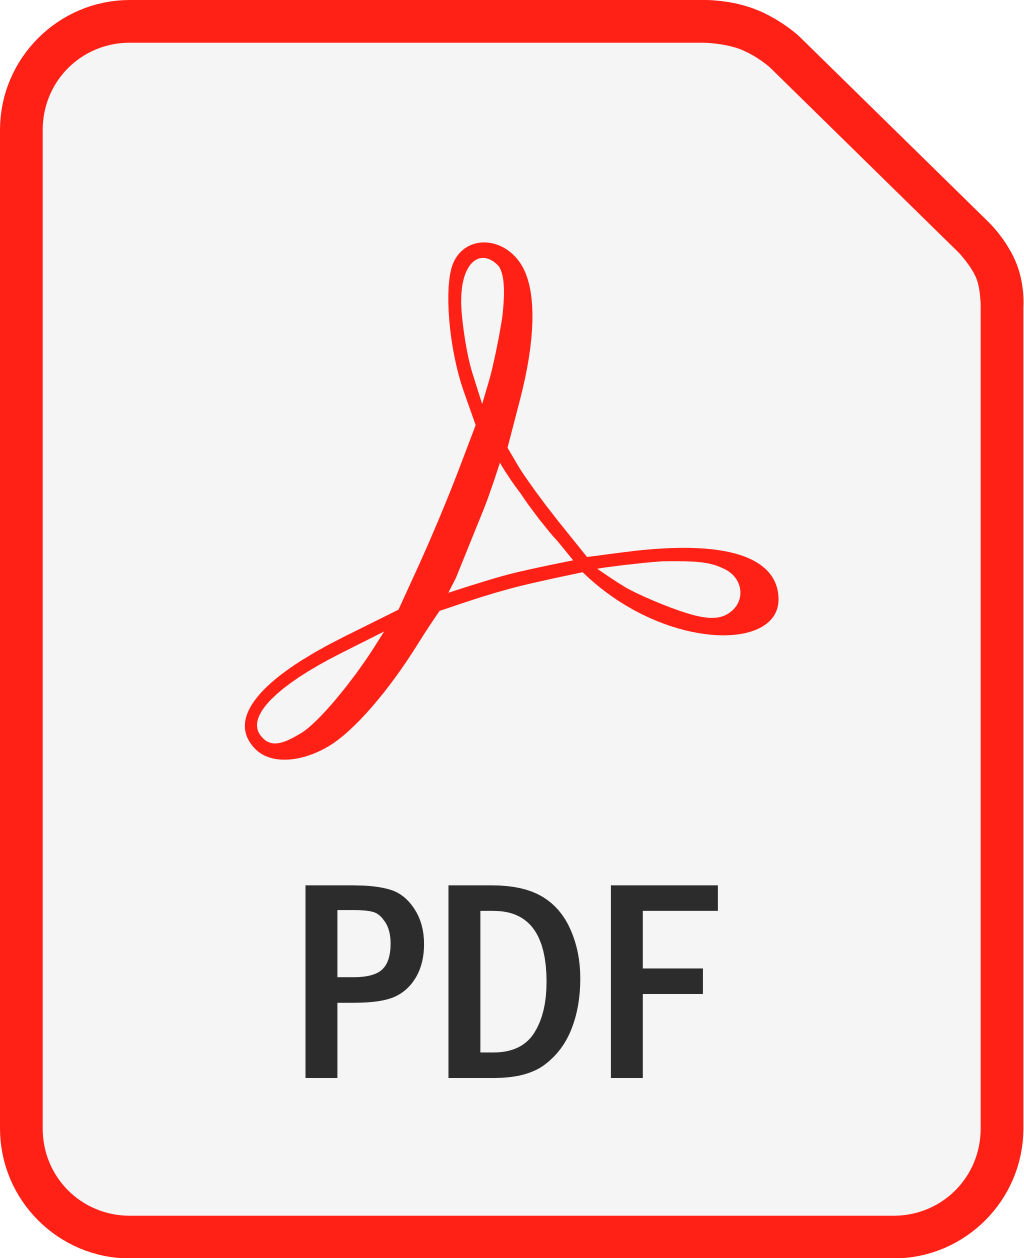
\includegraphics[scale=0.1]{"images/PDFfileIcon.png"}
	\caption{Adobe PDF Icon \cite{wiki-pdf-engl}}
	\label{fig:icon}
\end{figure}
